\section{Results and Discussion} \label{sec:results}
\subsection{Results}
An alpha level of 0.05 was used for all statistical tests. Two-way analysis of variance (ANOVA) tests were used to test all hypotheses. Both \xQ{} and \xO had two levels (`present', `absent').

\paragraph{\ref{itm:H1}---Total Score}
Box plots of the data are in Fig.~\ref{fig:score_box}. According to ANOVA all effects were statistically significant at $p<0.001$. Specifically, the main effect of \xQ{} yielded an F ratio of $F(1,1)=107.9, p<0.001$. The main effect of \xO{} yielded an F ratio of $F(1,1)=124.5,p<0.001$. The interaction effect was also significant $F(1,1)=26.4,p<0.001$.

Post-hoc comparisons using Tukey's HSD test revealed indicate that the \xQ{} `present' condition results in a significantly higher score than in control ($p<0.001$), the same for \xO{} `present' ($p<0.001$), and \xQ/\xO{} `present' ($p<0.001$). The condition \xQ{} `present' is not significantly different from \xO{} `present' ($p>0.05$), but the \xQ/\xO{} `present' condition is significantly higher than either \xQ{} `present' or \xO{} `present' conditions alone ($p<0.001$, and $p<0.01$ respectively).

\paragraph{\ref{itm:H2}---Trust}
Factor analysis of the survey questions indicated that questions 1,2,4,5,6, and 7 could be used in the same scale with a Cronbach's $\alpha = 0.83$. The Likert responses from these questions were combined by taking their average; this data is shown in Fig.~\ref{fig:time_box}. Analysis of variance indicated that the main effects of \xQ{} were significant $F(1,1)=13.6,p<0.001$. The main effects of \xO{} were also significant with $F(1,1)=7.3,p<0.01$. The interaction effect was not significant, $F(1,1)=0.05,p>0.05$.

In Post-hoc analysis using Tukey's HSD revealed that the \xQ{} `present' condition is significantly higher ($p<0.001$), as well as \xO{} `present' ($p<0.01$). The \xQ/\xO{} `present' condition is significantly higher than control as well ($p<0.001$). Other interactions were not significant.

\paragraph{\ref{itm:H3}---Average Task Time}
After analysis of the effects of \xQ{} and \xO{} on the average task time no effects were found to be significant with the main effect of \xQ{} yielding $F(1,1)=0.6,p>0.05$, \xO{} yielding $F(1,1)=0.1,p>0.05$ and the interaction effect yielding $F(1,1)=0.5,p>0.05$. 

       \begin{figure}[tb]
            \centering
            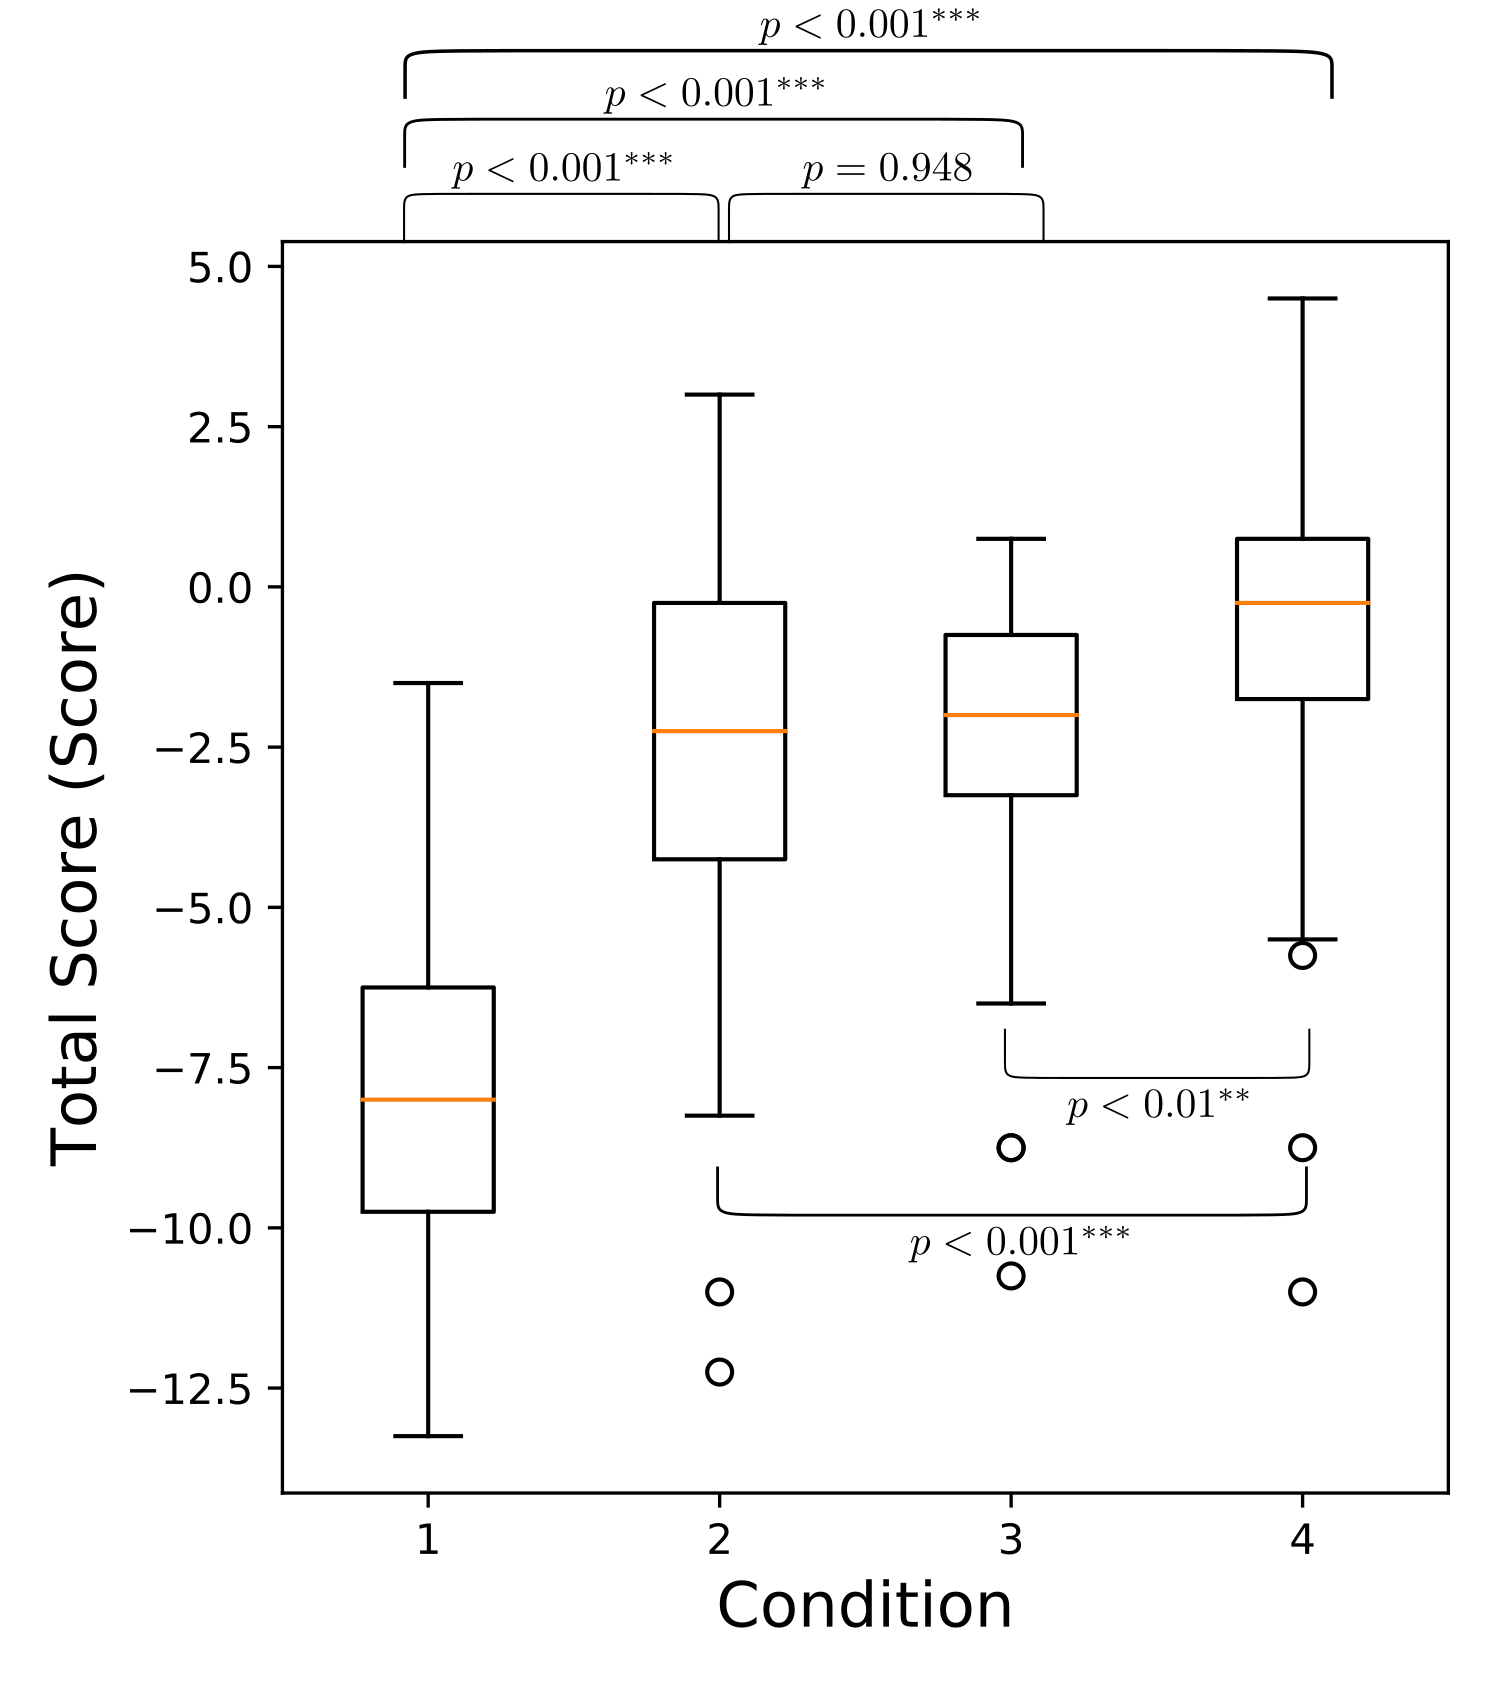
\includegraphics[width=0.8\linewidth]{Figures/total_score_box.png}
            \caption{Box plots showing the participants cumulative total score by condition.}
            \label{fig:score_box}
       \end{figure}
       \begin{figure}[tb]
            \centering
            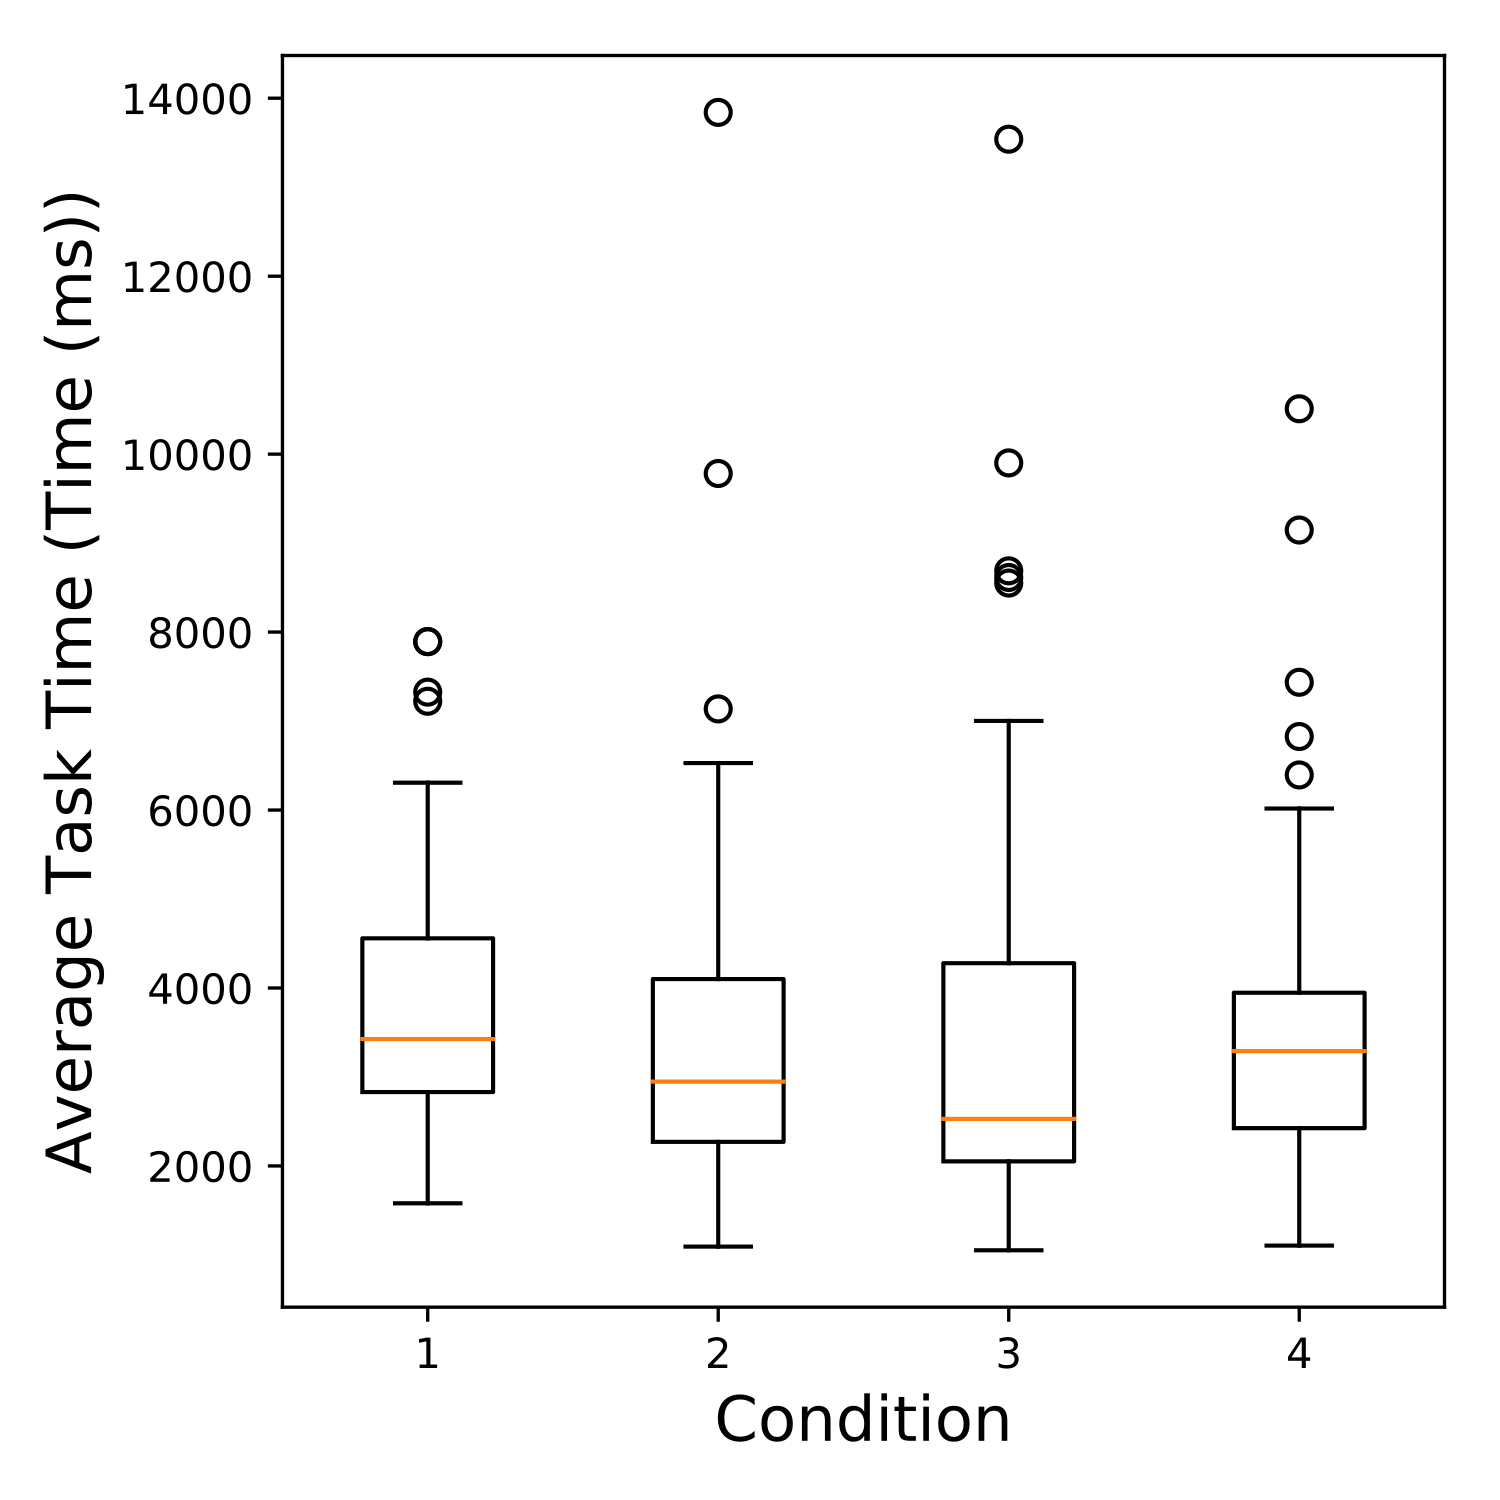
\includegraphics[width=0.8\linewidth]{Figures/avg_time_box.png}
            \caption{Box plots showing the participants average task time by condition.}
            \label{fig:time_box}
       \end{figure}
       \begin{figure}[tb]
            \centering
            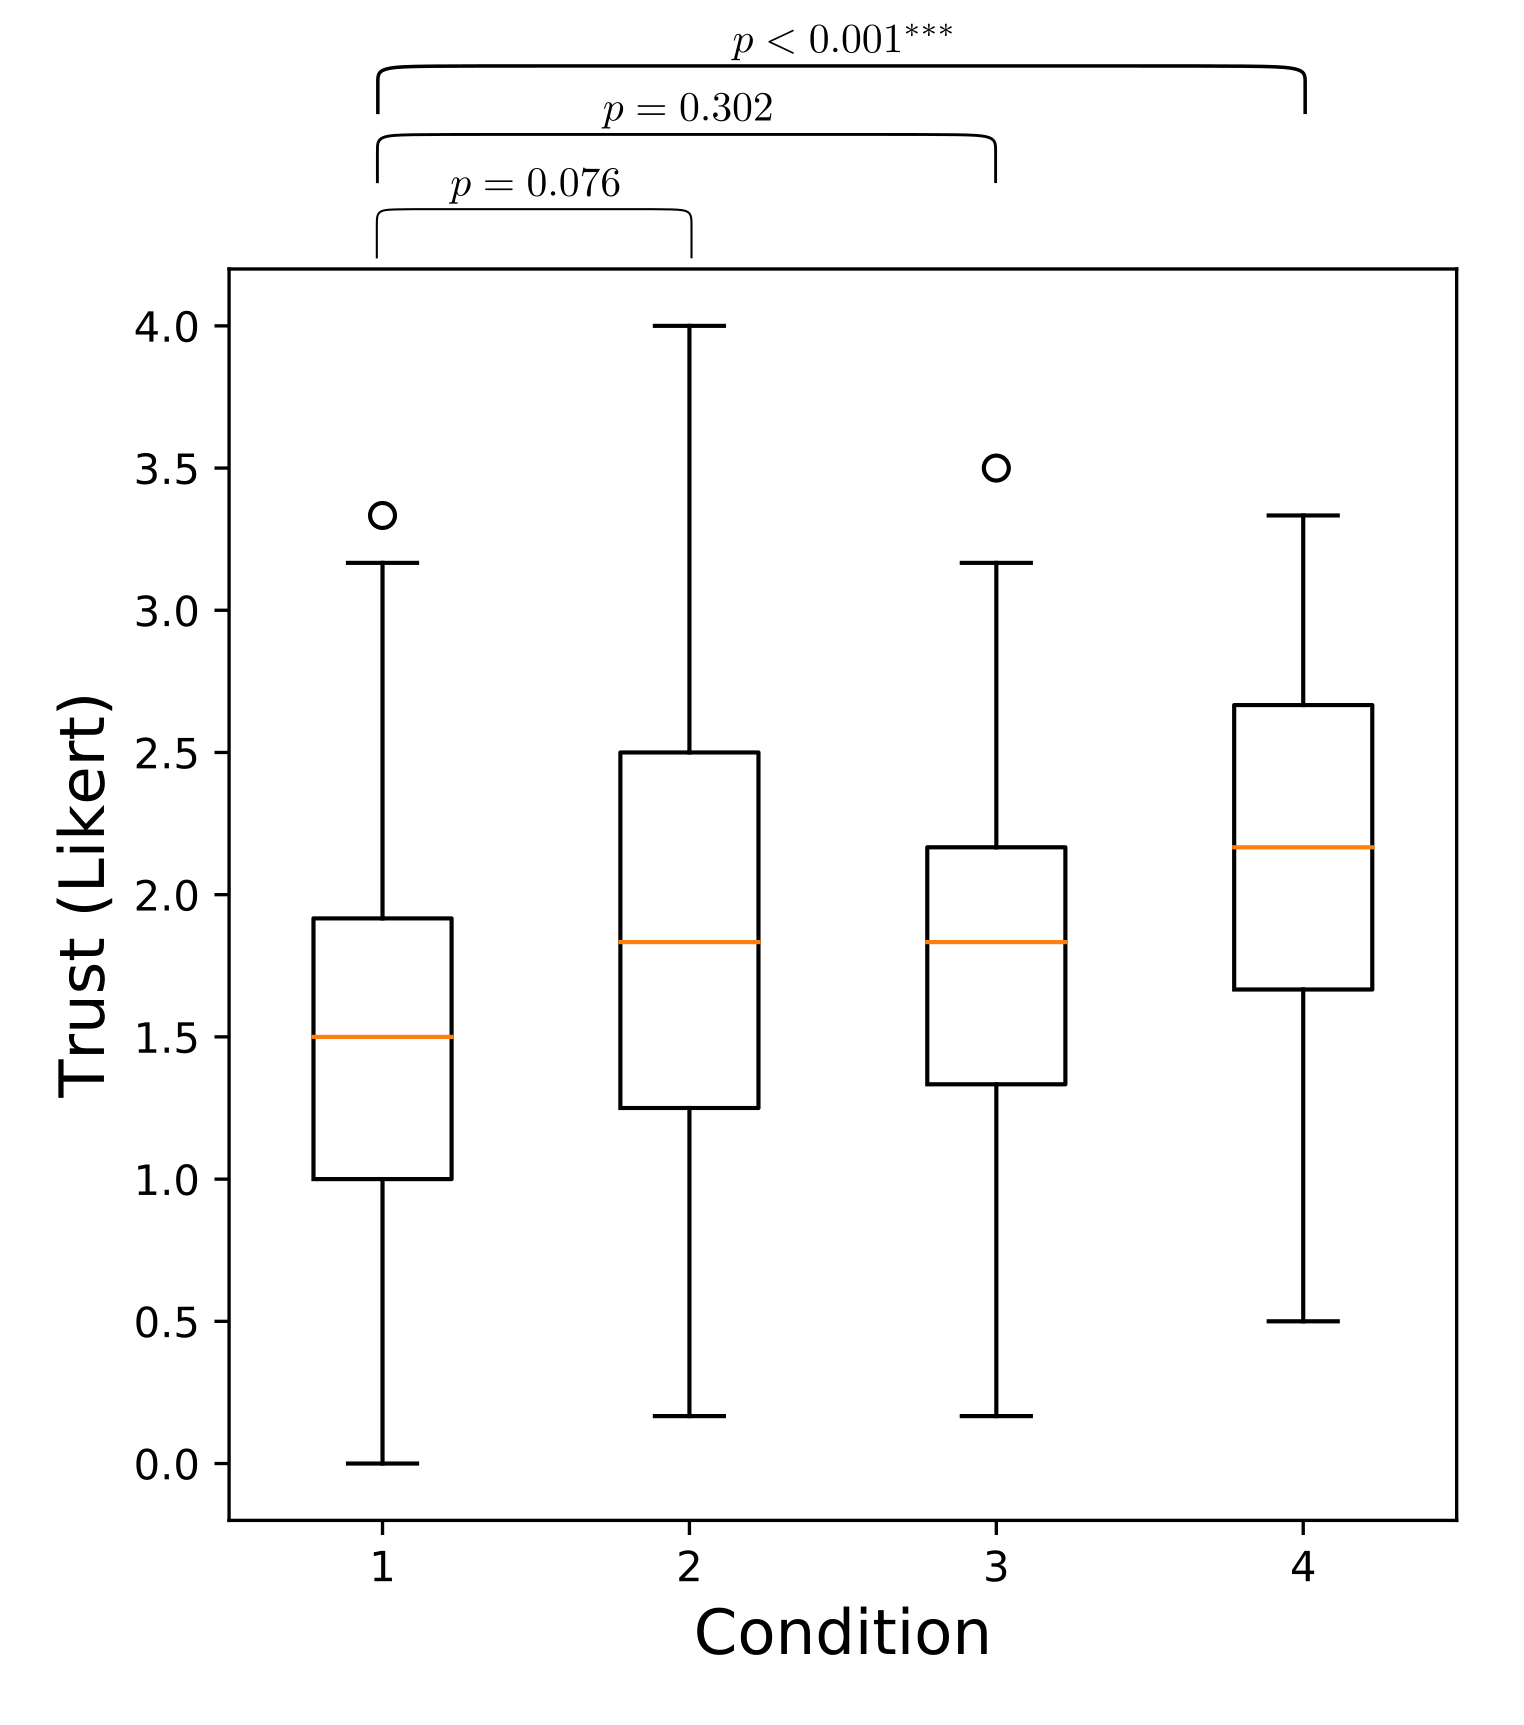
\includegraphics[width=0.8\linewidth]{Figures/trust_box.png}
            \caption{Box plots showing the participants trust by condition.}
            \label{fig:trust_box}
       \end{figure}

\subsection{Discussion}
The results show that the presence of \xQ{} and \xO{} helped the users to perform better on the task and get a higher total score. This was true individually in conditions 2 and 3 and even more so with both of the metrics `present'. This is impressive given the difficult nature of the task. A few different participants mentioned that they felt like ``the delivery truck should have been able to make more deliveries''. In co

The effects of self-confidence metrics on user trust while significant, were not as strong. Much of this can be attributed to the fact that this was a between-subjects study. Without a baseline experience it is hard for participants to gauge how much more they trust the UDT equipped with \xQ{} and/or \xO, but clearly their performance was better. The survey responses more likely reflect some of the biases that participants had regarding how they thought the UDT \emph{should have done}. A few participants shared that they felt the delivery truck should have been able to `do better', this indicates that they still felt like they didn't have enough information to really convince them that the UDT was really trustworthy. This suggests that users need to have the capability to understand more detail about the capabilities before they can be fully convinced (i.e. ``Solver Quality is low because the transition probability is very poor in this city'').

The fact that \xQ{} and \xO{} did not have a significant effect on the average time to complete tasks is somewhat surprising to us. This is due to the fact that both \xQ{} and \xO{} are meant to offload some of the decision-making work from the user. However, in reality \xQ{} and \xO{} are really presenting more nuanced information to the user that would not have considered before. For example, participants in the control condition likely had an implicit assumption that the UDT solver worked the same on every task (i.e. the latent \xQ{} was ``very good'' all of the time) since they had no real idea of any other possibility. Ultimately, further investigation is required to understand how user attention is shifting between these conditions.

These results are very promising in indicating that \famsec{} as an \emph{algorithmic assurance} elicits \emph{appropriate behavior}. User behaviors (indicated by decisions, and ultimately the score in this work) are really the objective measures of the effects of the assurances.

\brett{some interesting comments to possibly bring up}
Interesting comments: 1) \emph{``I felt like I had to decline the delivery too often''} 2) \emph{``I tried to figure it out from the map sometimes, but the truck was right more often than me''}, 3) \emph{``I thought that the proximity to the motorcycle gang would be a factor but it was very hard to predict''}, 4) \emph{``This feels rigged >.>''}, 5) \emph{``I enjoyed completing the HIT however the delivery truck should have been able to make more deliveries considering the short nature of the imagined route''} 5) \emph{``I think the system works well whenever it is trusted. I made the mistake of relying too much on the visible map. Things were better when using entire system.''}

As one participant noted: ``I think the system works well whenever it is trusted. I made the mistake of relying too much on the visible map. Things were better when using entire system.''
